%versi 2 (8-10-2016)
\chapter{Implementasi}
\label{chap:implementasi}
Pada bab ini akan dibahas implementasi \textit{API} yang digunakan untuk pembangunan situs. Bab ini juga akan membahas keputusan desain dan implementasi fitur-fitur yang ada secara mendalam.

\section{Persiapan Pembangunan Situs Pemesanan Tiket Kereta Api}

Dalam membangun situs pemesanan tiket kereta api ini, ada beberapa persiapan yang perlu dilakukan sebelum memulai pembangunan. Salah satu persiapannya adalah seperti yang sudah dijelaskan di \ref{sec:gdsapi} yaitu menyiapkan \textit{IP Address} untuk mengakses \textit{API}. Persiapan lainnya yaitu mempelajari alur pemesanan tiket kereta api \textit{online} dari sumber lain. Setelah mendapatkan gambaran alur pemesanan tiket kereta api dari berbagai sumber lain, pahami sistem penerbangan yang dipakai sekarang. Sistem penerbangan yang sudah ada mungkin memiliki bagian-bagian yang bisa dimanfaatkan kembali untuk menghemat waktu dan menjaga keseragaman fitur yang ada.

Terakhir, simpan semua bentuk respon \textit{API} ke kumpulan \textit{JSON file}. \textit{File} ini dibuat untuk berjaga-jaga jika \textit{API} yang ingin digunakan mengalami masalah. Dalam pembangunan proyek ini, ada kemungkinan \textit{API}-nya mengalami gangguan atau timbul masalah lain yang mencegah \textit{developer} untuk mengakses \textit{API} GDS. Oleh karena itu, perlu adanya rencana cadangan agar tidak terjadi proses saling menunggu yang mengakibatkan pembangunan web semakin tertunda.

\section{Pencarian Tiket Kereta Api}
\label{sec:pencariantiket} 
 
 Halaman pertama yang dibuat adalah halaman pencarian tiket kereta api. Halaman pencarian tiket menjadi halaman utama saat membuka proyek ini. Fungsi dari halaman mencari tiket adalah menerima masukan dari pengguna untuk kemudian diteruskan ke halaman selanjutnya. Masukan yang dimaksud di sini adalah stasiun awal, stasiun akhir, tanggal keberangkatan, tanggal pulang yang bersifat opsional, jumlah penumpang dan apakah pengguna memilih perjalanan 1 arah atau pulang pergi.
 
 Fitur yang ada di halaman ini sesuai dengan rancangan pada \ref{subsec:rancanganpencariantiket} antara lain adalah:
 
 \begin{enumerate}
     \item \textit{Auto-complete} untuk pemilihan stasiun.
     \item \textit{Date-picker} untuk pemilihan tanggal.
     \item Pengisian jumlah penumpang sesuai dengan aturan KAI secara otomatis.
 \end{enumerate}

Langkah pertama yang dilakukan adalah pembuatan fungsi \textit{model}. Daftar nama dan kode stasiun dari \textit{API} akan digunakan untuk \textit{auto-complete}. Untuk mempermudah \textit{debug} kedepannya, maka pembuatan \textit{model} dipisah menjadi 2. \textit{Model} yang hanya melakukan \textit{request} ke \textit{API} dan \textit{model} yang memiliki semua modul \textit{API}.

\textit{Model} pertama bernama \textit{TrainAPI\_GDS\_ model} dan bertugas untuk mengirimkan permintaan ke \textit{API}. \textit{Model} akan menerima \textit{URL} modul dan parameter yang diperlukan. Kemudian \textit{model} akan melakukan \textit{cURL} (melakukan \textit{request} ke sebuah \textit{URL} sesuai dengan \textit{parameter}) menggunakan \textit{URL} dan parameter yang diterima. Data kemudian diterima dan diperiksa. Jika terdapat eror dari hasil \textit{cURL} ke \textit{API}, dia akan menuliskan erornya ke \textit{log}. Jika tidak, data akan diproses seperti biasa.

\textit{Model} kedua adalah \textit{Train\_model} yang memberikan \textit{input} ke \textit{TrainAPI\_GDS\_model}. \textit{Model} ini dibuat semirip mungkin dengan \textit{API} untuk memudahkan permintaan data. \textit{Model} ini akan menerima respon dari \textit{API} dan mengembalikan datanya dalam bentuk data yang diperlukan oleh \textit{controller}.

Implementasi halaman pencarian tiket membutuhkan modul \textit{data/get-station-new}. Modul akan memberikan \textit{array} berisi daftar stasiun di Indonesia dengan nama dan kodenya. Contoh keluaran modul \textit{get station} dapat dilihat di \ref{subsec:getstation}. Data yang diterima akan digunakan untuk membantu pengguna memilih stasiun dengan menggunakan fitur pertama yaitu \textit{auto-complete}.

\textit{Controller} akan memanggil \textit{model} untuk mendapatkan daftar nama dan kode stasiun. Kemudian \textit{controller} akan menyiapkan data-data lain yang dibutuhkan oleh \textit{view}. \textit{View} membutuhkan data seperti \textit{default value} dan jenis penumpang.

\textit{View} akan memiliki tampilan yang mirip dengan bagian penerbangan untuk konsistensi. Tampilan dari bagian kereta akan menggunakan beberapa bagian dari penerbangan. Tampilan untuk halaman kereta tentunya berbeda dengan tampilan pada halaman pesawat. Oleh karena itu, butuh beberapa penyesuaian di \textit{view} halaman pencarian tiket kereta.

\begin{figure}[H]
        \center
        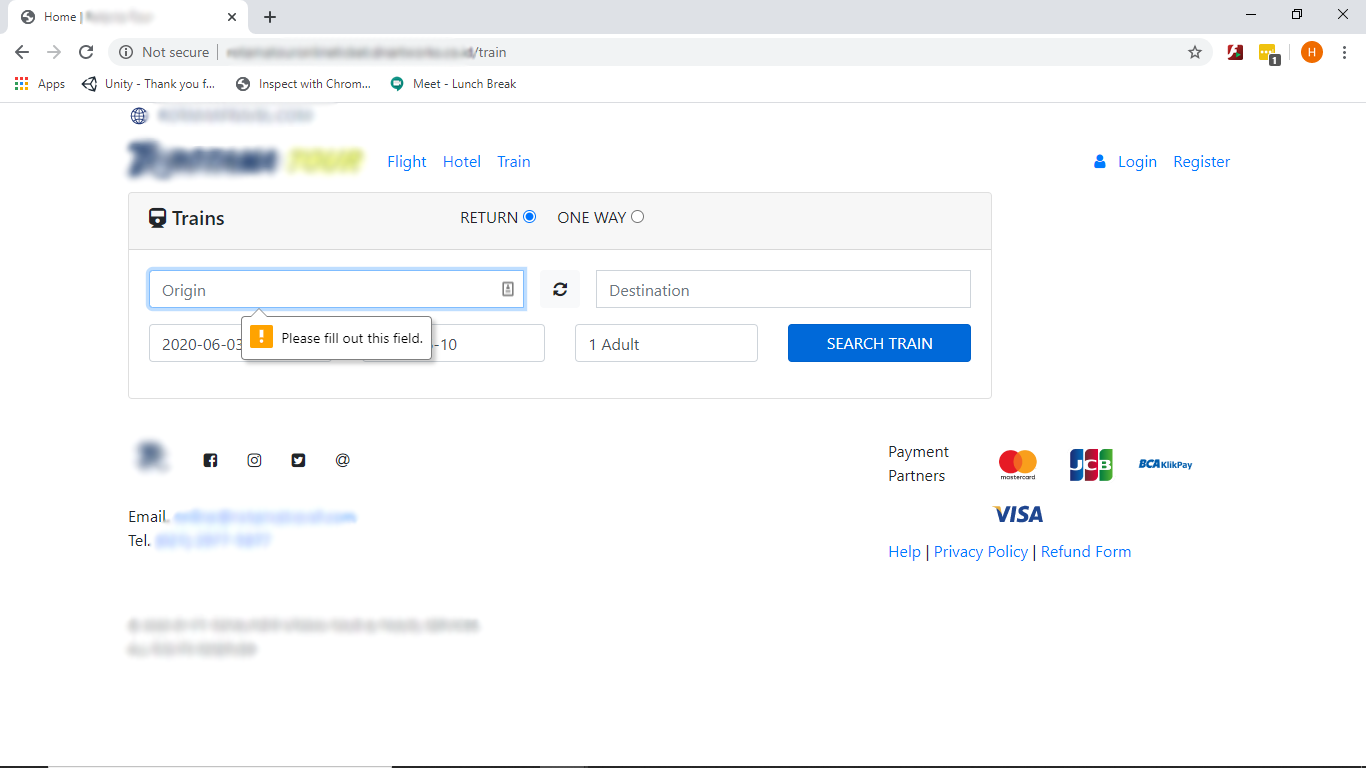
\includegraphics[width=\textwidth,height=\textheight,keepaspectratio]{Gambar/Search train no data pencarian tiket.png}
        \caption{Hasil Implementasi Halaman Pencarian Tiket.}
            \label{img:hasilimplementasicaritiket}
        \end{figure}

Penyesuaian pertama ada di sisi tampilan. Perubahan pertama adalah merubah setiap unsur penerbangan menjadi kereta. Perubahan lainnya adalah menghapus kelas dari salah satu \textit{input} seperti dapat dilihat pada gambar \ref{img:hasilimplementasicaritiket}. Kelas dihapus karena di pemilihan jadwal kereta, kelas dan sub-kelas sudah ditampilkan di sana.

Penyesuaian berikutnya adalah fitur \textit{auto-complete}. Fitur \textit{auto-complete} bandara dan kereta memiliki sumber yang berbeda. Oleh karena itu, \textit{auto-complete} harus diubah mengikuti kereta.

\textit{Auto-complete} di halaman ini menggunakan \textit{typeahead} milik \textit{bootstrap}. \textit{Bootstrap} adalah \textit{framework} untuk \textit{css}. \textit{Typeahead} memiliki parameter \textit{source} yang digunakan untuk menjadi sumber \textit{auto-complete}. Data stasiun yang dikirimkan oleh \textit{controller} akan menjadi \textit{source} untuk \textit{typeahead}. 

Data stasiun yang menjadi sumber \textit{typeahead} harus diolah dulu agar mempermudah pencarian. Jika langsung menggunakan sumber dari \textit{controller} tanpa diolah, data yang menjadi sumber adalah nama atau kode stasiun. Oleh karena itu, data yang akan menjadi sumber diubah dulu dengan format nama (kode).

Setelah mendapatkan sumber yang diinginkan, langkah selanjutnya adalah menentukan data apa yang digunakan untuk \textit{auto-complete}. \textit{Typeahead} memiliki 2 \textit{function} yang dimanfaatkan untuk halaman ini yaitu \textit{afterSelect} yang dipakai saat data sudah dipilih dan \textit{matcher} yang dipakai untuk memberikan pilihan \textit{auto-complete}. Fungsi \textit{afterSelect} dipakai untuk menyiapkan \textit{input} untuk halaman selanjutnya. Fungsi \textit{matcher} dipakai untuk memberikan pilihan kemungkinan stasiun yang diinginkan pengguna. Dalam fungsi \textit{matcher} perlu ditambahkan kode agar tidak memunculkan stasiun yang sama untuk stasiun keberangkatan dan tujuan saat pengguna mengetik. Di \textit{matcher} juga perlu dispesifikasikan saat return bahwa \textit{auto-complete} bisa menggunakan nama atau kode yang dalam implementasi ini dilakukan saat akan melakukan \textit{return}.

Fitur kedua adalah \textit{date-picker}. Fungsi \textit{datepicker} memberikan format pemilihan tanggal kepada pengguna. Dalam pengimplementasian, hari di \textit{datepicker} menggunakan bahasa inggris. Opsi yang digunakan untuk \textit{datepicker} adalah format tanggal yyyy-mm-dd, \textit{datepicker} langsung ditutup saat tanggal dipilih, tidak memunculkan \textit{keyboard} di \textit{mobile}, menampilkan maksimal hanya sampai bulan, dan tanggal yang bisa dipilih mulai dari tanggal hari pengguna menggunakan web. Tanggal mendapatkan nilai \textit{default} dari \textit{controller} yaitu seminggu dari hari halaman dibuka untuk tanggal keberangkatan dan seminggu dari tanggal keberangkatan untuk tanggal pulang mengikuti penerbangan.

Fitur terakhir adalah jumlah penumpang. Jumlah maksimal penumpang yang bisa memesan tiket adalah 4 orang untuk setiap pemesanan. Jumlah penumpang bayi tidak boleh melebihi jumlah penumpang dewasa. Dalam implementasinya, penumpang dewasa dibuat tidak bisa melebihi 4 orang. Setiap jumlah dewasa dan bayi melebihi 4 orang maka jumlah bayi akan menurun mengikuti jumlah maksimal dikurangi jumlah dewasa. Jika jumlah penumpang bayi dan jumlah penumpang dewasa sama, saat jumlah penumpang dewasa dikurangi, maka jumlah penumpang bayi juga berkurang mengikuti jumlah penumpang dewasa.

Saat tombol \textit{search train} ditekan, data akan dikirim dari \textit{view} ke \textit{controller} dengan metode \textit{get}. Data dikirimkan menggunakan \textit{get} karena parameter pencarian tidak bersifat rahasia. Selain itu, mengirim menggunakan \textit{get} mempermudah implementasi pada tahap berikutnya. Dengan menggunakan \textit{get}, jika pengguna ingin memuat ulang halaman selanjutnya, parameter pencarian sudah tersimpan di \textit{URL} sehingga tidak perlu implementasi lanjutan.

\section{Pemilihan Jadwal Kereta Api}
\label{sec:pemilihanjadwal}

Halaman kedua adalah halaman pemilihan jadwal kereta api. Halaman ini menampilkan jadwal-jadwal kereta api sesuai dengan parameter masukan di halaman sebelumnya. Di halaman ini, pengguna bisa melihat dan memilih jadwal kereta api yang pengguna inginkan. Halaman ini menyediakan fitur filter untuk mempermudah pengguna memilih jadwal sesuai kondisi yang pengguna inginkan. 

\begin{figure}[H]
        \center
        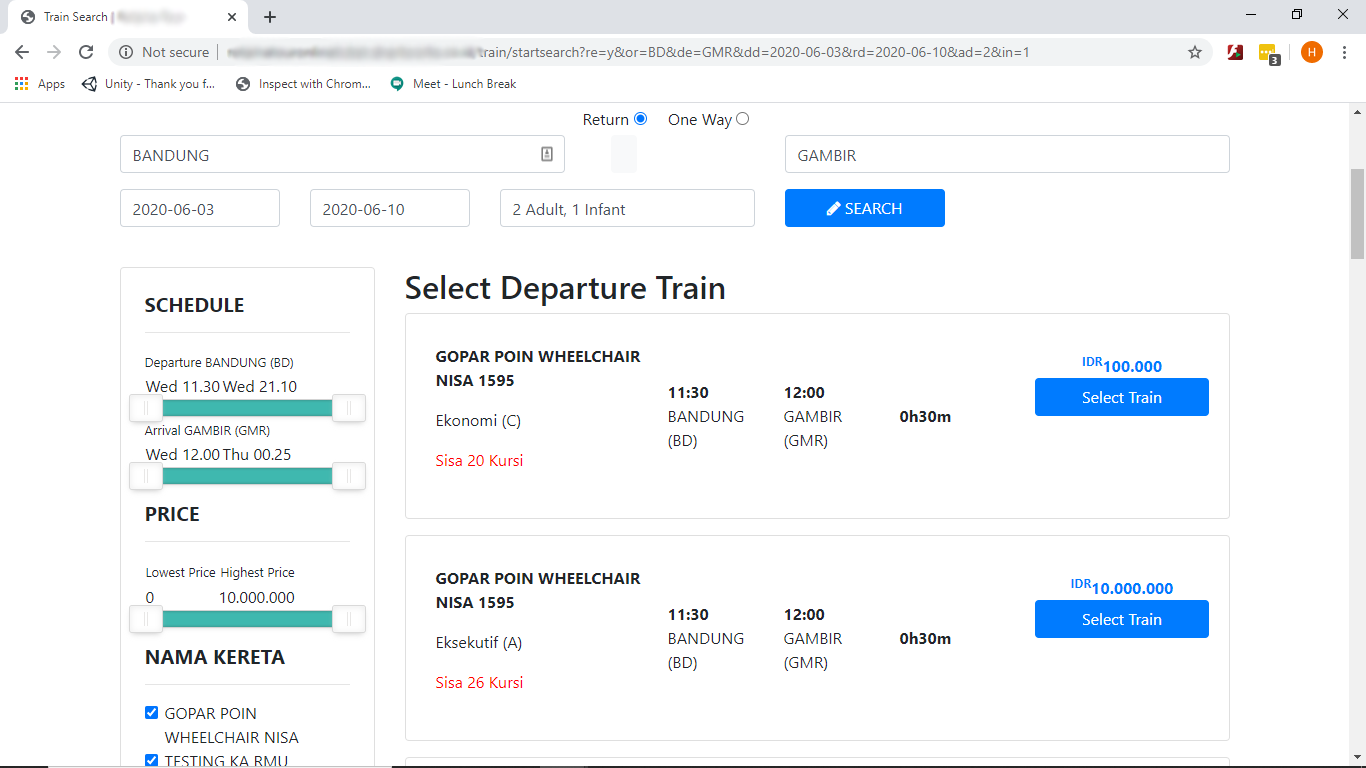
\includegraphics[width=\textwidth,height=\textheight,keepaspectratio]{Gambar/Search result pilih jadwal berangkat.png}
        \caption{Hasil Implementasi Halaman Pemilihan Jadwal.}
            \label{img:implementasijadwalberangkat}
        \end{figure}

Kotak pencarian jadwal yang ada di halaman pertama kembali ditampilkan di halaman ini seperti yang dapat dilihat pada gambar \ref{img:implementasijadwalberangkat}. Tujuan dari dimasukkannya kembali fitur pencarian jadwal adalah agar pengguna dapat langsung melakukan pencarian kembali jika hasil pencarian kosong. Selain itu, parameter \textit{input} yang dimasukkan pengguna juga ditampilkan kembali di sini sehingga pengguna dapat memeriksa kesesuaian pencarian. Pengguna juga tidak perlu memasukkan \textit{input} yang sama berulang-ulang jika pengguna hanya ingin mengganti beberapa parameter.

Halaman ini menampilkan hasil pencarian dengan informasi-informasi jadwal kereta dan filter untuk mempermudah pengguna memilih. Informasi yang ada pada setiap jadwal adalah nama dan nomor kereta api, kelas dan sub-kelas, ketersediaan kursi, jam keberangkatan dan tujuan beserta stasiunnya, lama perjalanan dan harga. Selain itu, di sebelah hasil pencarian terdapat 3 filter berbeda. Filter-filter tersebut adalah berdasarkan waktu, harga dan nama kereta.

Jika pengguna memilih perjalanan pulang pergi, maka halaman ini akan menampilkan jadwal keberangkatan terlebih dahulu. Jadwal pulang akan disembunyikan sampai pengguna sudah memilih jadwal berangkat. Saat pengguna sudah memilih jadwal berangkat, jadwal berangkat sisanya akan disembunyikan dan diganti dengan jadwal pulang seperti pada gambar \ref{img:implementasijadwalpulang}. Jadwal berangkat yang dipilih akan tetap ditampilkan di atas jadwal pulang.

\begin{figure}[H]
        \center
        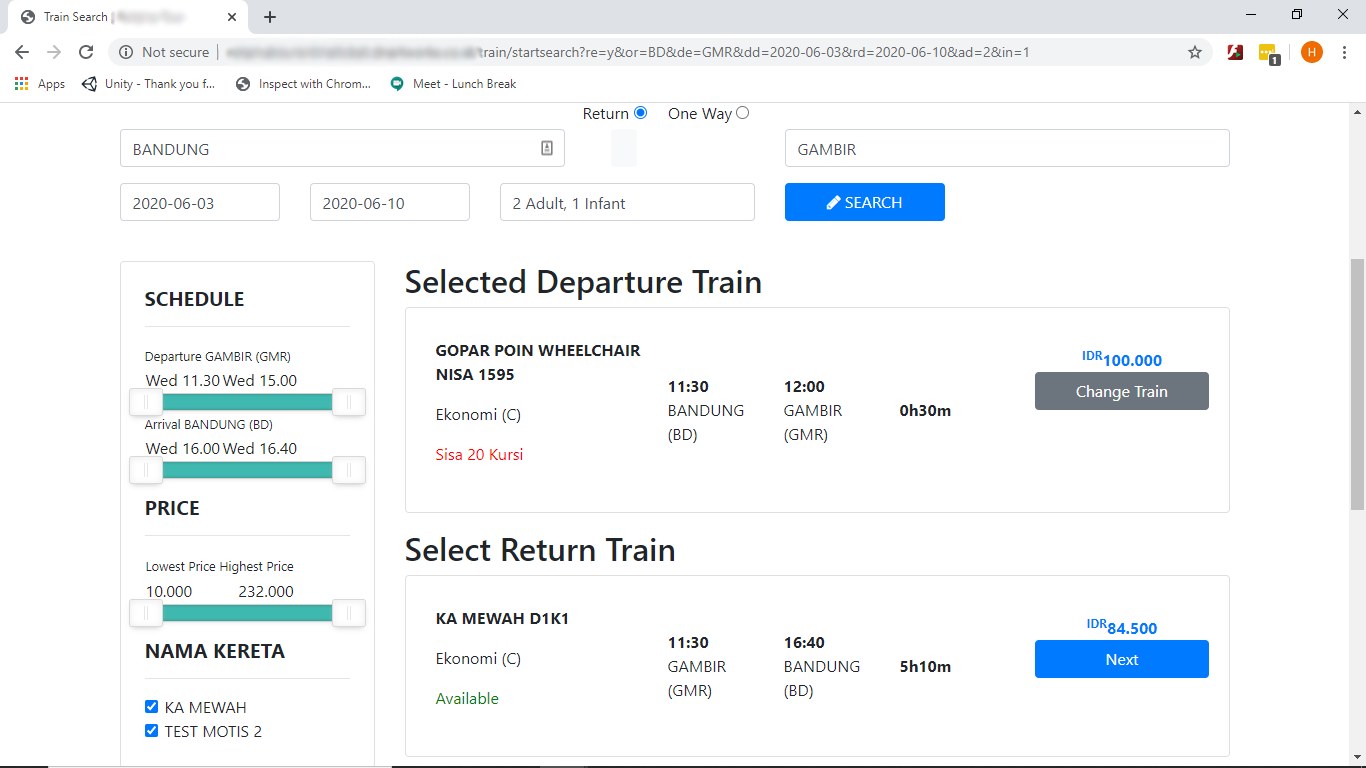
\includegraphics[width=\textwidth,height=\textheight,keepaspectratio]{Gambar/Search result pilih jadwal pulang.png}
        \caption{Hasil Implementasi Halaman Pemilihan Jadwal Perjalanan Pulang Pergi.}
            \label{img:implementasijadwalpulang}
        \end{figure}

Tombol memilih kereta berubah bergantung pada apakah pengguna memilih perjalanan 1 arah atau pulang pergi. Jika pengguna memilih perjalanan satu arah, tombol akan bertuliskan \textit{next} dan memunculkan \textit{pop-up} untuk konfirmasi dan lanjut ke halaman selanjutnya jika ditekan. Jika pengguna memilih perjalanan pulang pergi, maka tombol akan bertuliskan \textit{select train} yang jika ditekan, akan menampilkan jadwal pulang dan menyimpan jadwal yang dipilih di atas jadwal pulang. Tombol \textit{change train} akan menghilangkan jadwal yang dipilih dan menampilkan kembali jadwal keberangkatan.

Filter yang digunakan untuk membantu memilih adalah filter waktu, harga dan nama kereta. Ketiga filter ini merupakan filter yang ada juga di penerbangan. Filter waktu dan harga menggunakan \textit{slider} untuk melakukan penyaringan. \textit{Slider} memudahkan pengguna untuk mengeliminasi jadwal-jadwal di luar jangkauan \textit{slider}. Filter nama kereta menggunakan \textit{checkbox} karena pengguna dapat melihat daftar kereta yang ada dan langsung memilih satu per satu kereta yang ditampilkan.

Halaman ini menggunakan modul \textit{information/get-rail-schedule-new} untuk mendapatkan jadwal sesuai masukan dari pengguna. Data diambil dari \textit{API} menggunakan kedua model yang sudah dibuat dan dijelaskan di \ref{sec:pencariantiket}. Metode baru ditambahkan kepada \textit{Train\_model} untuk mendapatkan data yang diperlukan. Metode ini akan mengembalikan jadwal kereta seperti yang dapat dilihat pada \ref{subsec:getrailschedule}.

\textit{Controller} untuk halaman ini memiliki 3 \textit{function} yaitu menampilkan halaman pemilihan jadwal, melakukan pencarian jadwal dan membuat format data hasil pencarian untuk \textit{view}. Fungsi pertama akan menerima masukan dari halaman pertama dan meneruskan ke \textit{view}. Fungsi kedua akan dipanggil di \textit{view} dan akan mendapatkan hasil pencarian. Hasil pencarian akan diteruskan ke fungsi ketiga sehingga bisa ditampilkan dengan rapi di \textit{view}.

Fungsi pertama menerima \textit{input} dari halaman pertama saat tombol \textit{search train} ditekan. \textit{Endpoint} yang akan diproses di \textit{view} disiapkan di sini. Data-data lain seperti menampilkan \textit{input} kembali di kotak pencarian diproses di sini. Fungsi pertama memisahkan menampilkan tampilan dan pencarian sehingga pengguna tidak menunggu lama pada halaman pertama dan berpikiran halaman tidak responsif.

\begin{figure}[H]
        \center
        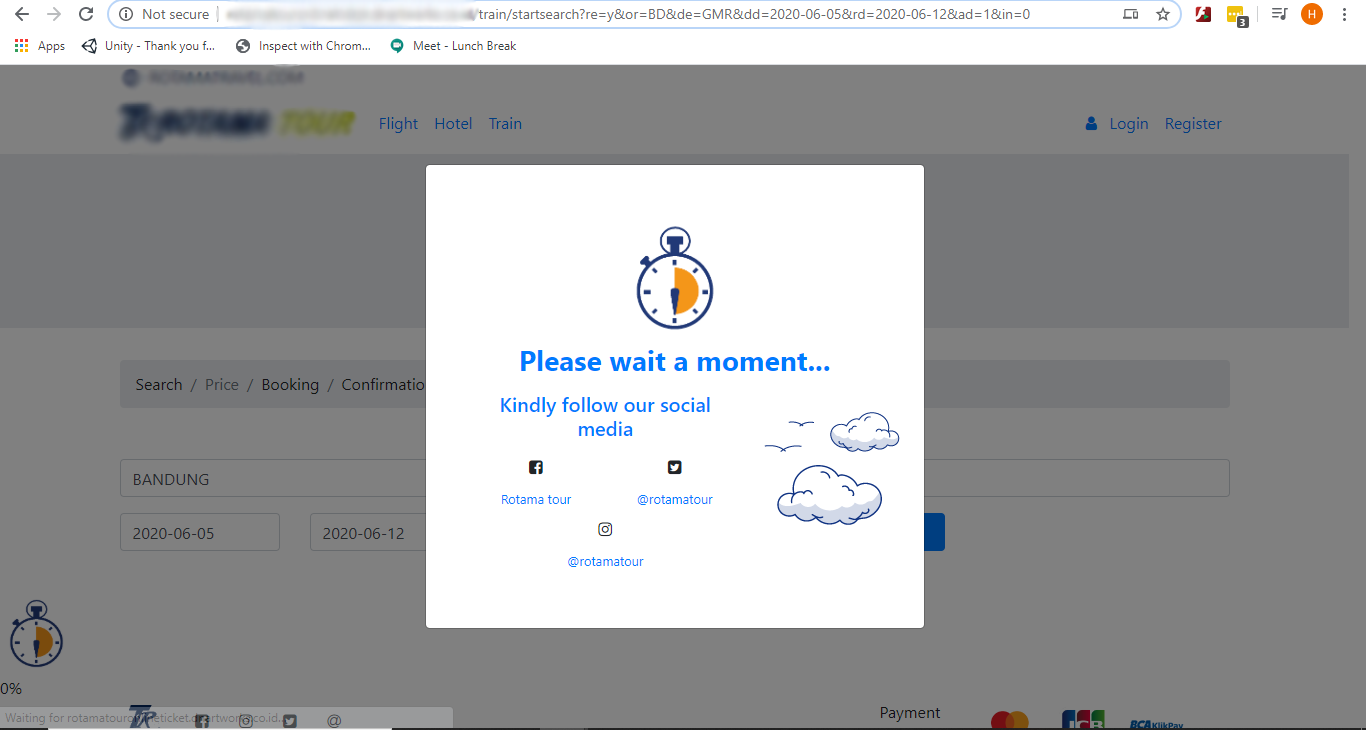
\includegraphics[width=\textwidth,height=\textheight,keepaspectratio]{Gambar/Loading pilih jadwal.png}
        \caption{\textit{Loading Screen} Halaman Pemilihan Jadwal.}
            \label{img:loadingpilihjadwal}
        \end{figure}

Fungsi kedua dipanggil di \textit{view} saat halaman sudah ditampilkan. Pencarian akan dilakukan saat layar menunjukkan \textit{loading} seperti pada gambar \ref{img:loadingpilihjadwal}. Fungsi ini meminta hasil pencarian jadwal lewat \textit{Train\_model} seperti pada pencarian tiket. Hasil yang didapatkan akan diteruskan ke fungsi ketiga agar bisa ditampilkan di \textit{view}.

Fungsi ketiga memberikan format pada hasil pencarian. Pada fungsi ini, data-data yang dibutuhkan di \textit{view} disiapkan. Data yang dimaksud adalah data seperti jarak filter, nama-nama kereta dan informasi-informasi jadwal. Hasil format dikembalikan ke fungsi kedua untuk ditampilkan di \textit{view}.

\textit{View} untuk halaman ini terpisah menjadi 2. \textit{View} pertama adalah keseluruhan halaman yang ditampilkan begitu tombol \textit{search train} ditekan. \textit{View} kedua adalah bagian halaman yang menampilkan hasil pencarian. \textit{Loading screen} akan ditampilkan selama \textit{view} kedua belum siap.

\textit{View} pertama memiliki isi yang kurang lebih sama dengan halaman pencarian tiket karena halaman ini masih memiliki kotak pencarian. Perbedaan di sini adalah penggantian nilai \textit{default} dengan masukan yang sudah ada. \textit{View} pertama juga menampilkan \textit{loading screen} sambil menunggu pencarian selesai dilakukan. Saat menampilkan \textit{loading screen}, \textit{view} akan memanggil \textit{endpoint} yang didapat dari \textit{controller}. \textit{Endpoint} itu berisi \textit{URL} yang mengarah ke fungsi kedua \textit{controller} di halaman ini. 

Pengaturan filter dilakukan di \textit{view} pertama. Filter baru akan mendapatkan data yang diperlukan saat pencarian selesai dilakukan. Filter akan diinisialisasi terlebih dahulu dengan kondisi awal menampilkan semua jadwal yang ada. Harga dan waktu menggunakan \textit{nouislider} dari javascript sementara nama kereta menggunakan \textit{dropbox} biasa. Setiap kali filter berubah, maka hasil akan disaring ulang memastikan jadwal mana yang sesuai dan yang tidak.

\textit{View} kedua adalah tampilan hasil pencarian yang dapat dilihat di bawah kotak pencarian. \textit{View} ini yang mengatur jadwal mana yang ditampilkan dan disembunyikan. Posisi informasi yang ditampilkan di masing-masing jadwal juga diatur di sini. Saat tombol \textit{next} ditekan dan pengguna sudah menkonfirmasi di \textit{pop-up}, pengguna akan diarahkan ke halaman selanjutnya.

\section{Pengisian Informasi Penumpang}
\label{sec:pengisianinfopenumpang}

Halaman ketiga adalah halaman pengisian informasi penumpang. Halaman ini menampilkan \textit{form} untuk mengisi data pemesan dan penumpang. Selain itu, halaman ini juga menampilkan \textit{sidebar} yang memuat informasi dari jadwal yang sudah dipilih. Halaman ini memiliki 2 tombol di bawah yang mengarahkan pengguna ke halaman pemilihan kursi atau halaman konfirmasi.

\begin{figure}[H]
        \center
        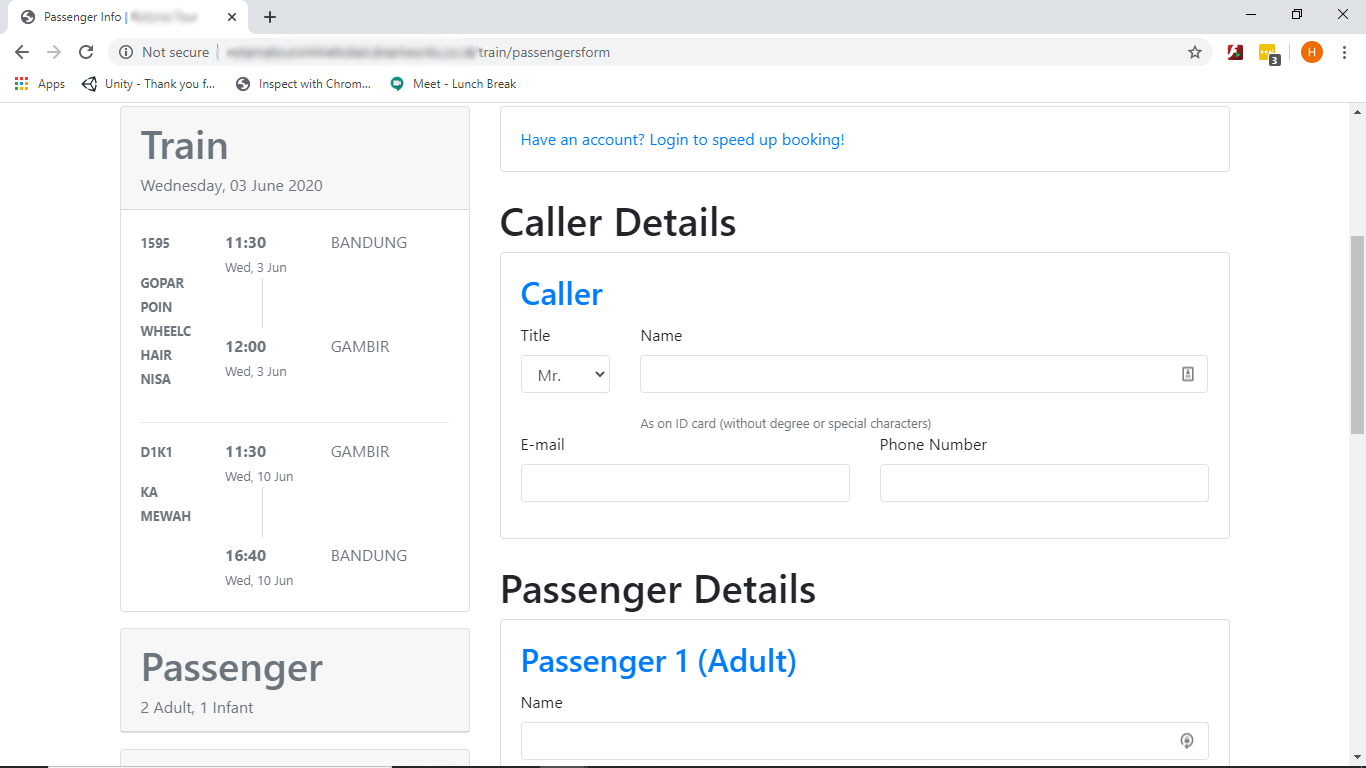
\includegraphics[width=\textwidth,height=\textheight,keepaspectratio]{Gambar/Sidebar isi data 1.png}
        \caption{Halaman Pengisian Data 1.}
            \label{img:isidata1}
        \end{figure}
        
        
Halaman pengisian informasi penumpang memiliki 2 \textit{form} dengan tujuan berbeda. \textit{Form} pertama adalah untuk mengisi data pemesan. Data pemesan dibutuhkan sebagai orang yang dapat dihubungi terkait pemesanan. Data yang dibutuhkan dari pemesan adalah \textit{title (Mr., Mrs., Ms)}, nama, email dan nomor telepon seperti yang dapat dilihat pada gambar \ref{img:isidata1}. \textit{Form} kedua adalah pengisian data penumpang. Pengisian data penumpang langsung memiliki kategori untuk membedakan data penumpang dewasa dan bayi. Data yang dibutuhkan oleh kedua kategori ini sama yaitu nama dan identitas. Identitas yang dimaksud adalah nomor KTP atau KK  seperti yang dapat dilihat pada gambar \ref{img:isidata2}.

\begin{figure}[H]
        \center
        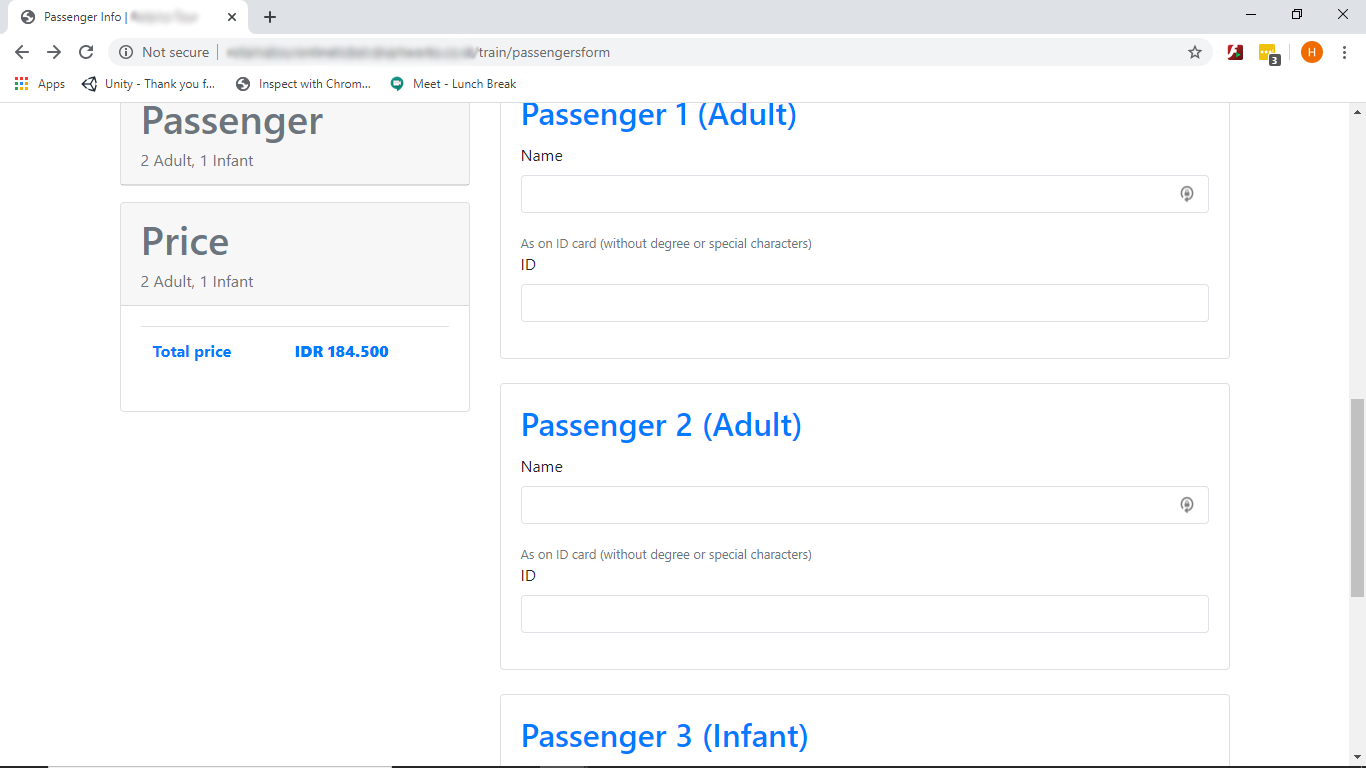
\includegraphics[width=\textwidth,height=\textheight,keepaspectratio]{Gambar/Sidebar isi data 2.png}
        \caption{Halaman Pengisian Data 2.}
            \label{img:isidata2}
        \end{figure}

\begin{figure}[H]
        \center
        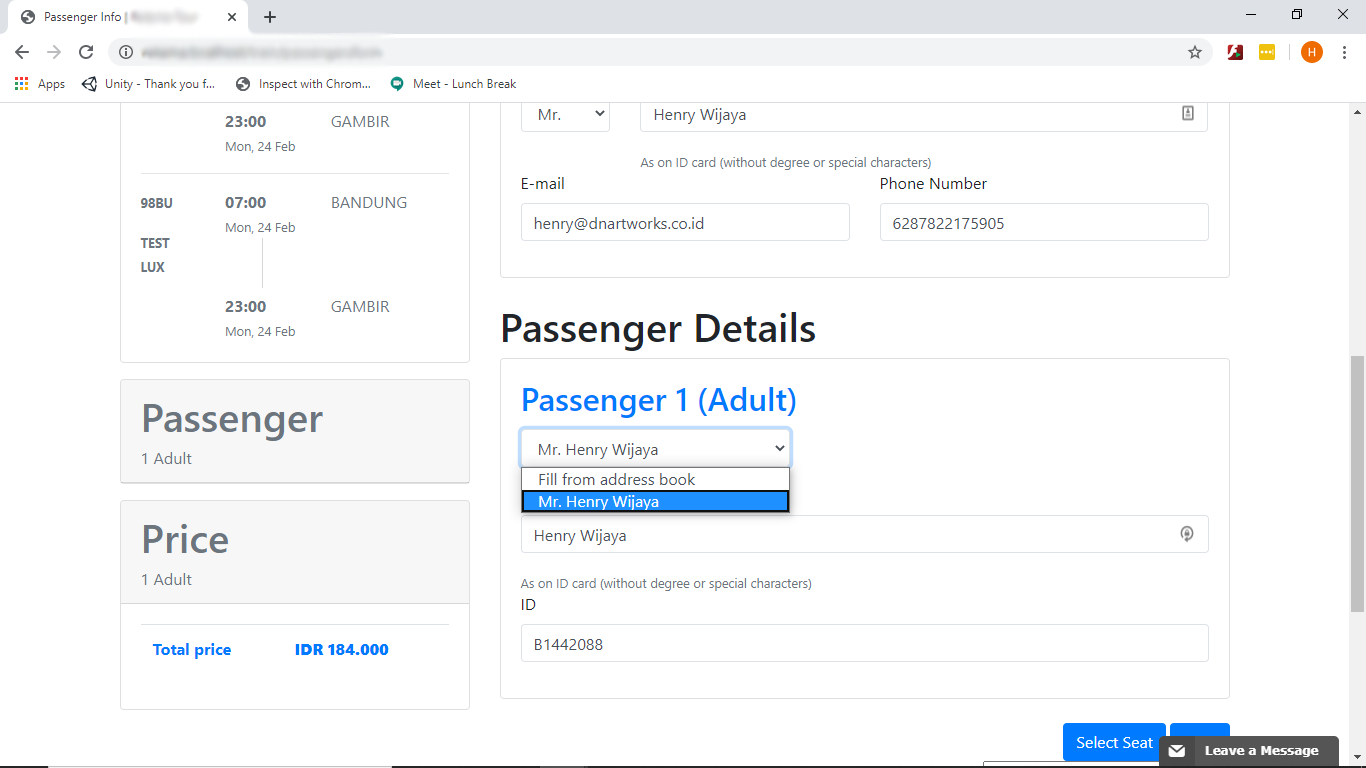
\includegraphics[width=\textwidth,height=\textheight,keepaspectratio]{Gambar/Fill from address book isi data.png}
        \caption{\textit{Fill from Address Book} Halaman Pengisian Data.}
            \label{img:fillfromisidata}
        \end{figure}

Halaman ini menyediakan fitur untuk mengisi data secara otomatis jika pengguna sudah terdaftar. Jika pengguna belum \textit{login}, terdapat tautan yang dapat ditekan di atas \textit{form} pengisian data pemesan. Tautan tersebut akan mengarahkan pengguna ke \textit{login screen}. Setelah pengguna berhasil \textit{login}, pengguna akan kembali ke halaman ini dan dapat menggunakan fitur \textit{fill from address book}. Dengan memilih orang yang terdapat pada \textit{dropbox}, data akan diisi secara otomatis sesuai data yang sudah ditambahkan di akun pengguna seperti yang dapat dilihat pada gambar \ref{img:fillfromisidata}.

Halaman ini menggunakan \textit{User\_model} yang sudah ada dari sistem sebelumnya. Dengan menggunakan \textit{User\_model}, pengisian data secara otomatis dapat dilakukan. Data yang diisi di \textit{form} halaman ini akan digunakan di \textit{Train\_model} saat tombol ditekan. Modul yang diperlukan adalah modul \textit{transaction/booking-rail-new} yang dapat dilihat detailnya di \ref{subsec:bookingrail}. Pada tahap ini, \textit{model} pertama harus diubah karena sebelumnya, \textit{cURL} yang dilakukan tidak menerima parameter berupa \textit{array} sehingga dibutuhkan sedikit penyesuaian di \textit{TrainAPI\_GDS\_Model}.

Halaman ini menambahkan 2 fungsi baru pada \textit{controller}. Fungsi pertama adalah menampilkan halaman pengisian data. Fungsi kedua adalah fungsi yang menggunakan \textit{model} seperti yang dijelaskan di paragraf sebelumnya. Fungsi kedua terletak di tombol \textit{select seat} dan \textit{next} di bawah yang dapat dilihat di \ref{img:fillfromisidata}.

Fungsi pertama halaman ini akan menerima data dari halaman sebelumnya dan mengolah datanya untuk ditampilkan di \textit{sidebar}. Data jadwal yang diolah akan dipresentasikan di samping dengan informasi jadwal, jumlah penumpang dan harga. Data tersebut akan dipakai di potongan \textit{view sidebar} yang ditempelkan pada halaman pengisian data. Selain itu, jenis dan jumlah penumpang akan memengaruhi tampilan \textit{form} pengisian data penumpang. 

Fungsi kedua adalah fungsi yang mengarahkan pengguna ke halaman selanjutnya. Fungsi ini menggunakan \textit{Train\_model} untuk mendapatkan kode \textit{booking} yang akan digunakan di halaman selanjutnya. Saat fungsi ini mengarahkan pengguna, tombol yang ditekan pengguna akan diperiksa terlebih dahulu. Jika pengguna menekan tombol \textit{select seat}, maka pengguna akan diarahkan ke halaman pemilihan kursi. Jika pengguna menekan tombol \textit{next}, maka pengguna akan diarahkan ke halaman konfirmasi.

\begin{figure}[H]
        \center
        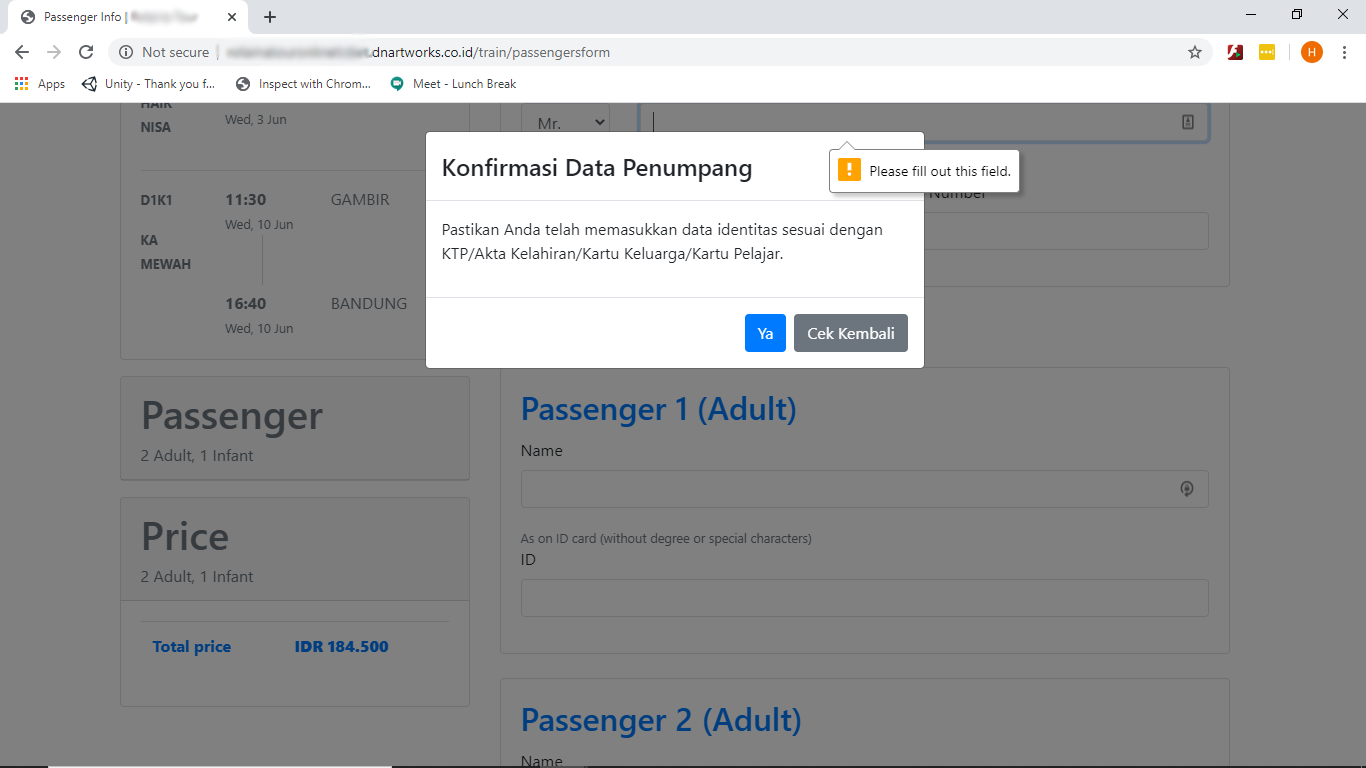
\includegraphics[width=\textwidth,height=\textheight,keepaspectratio]{Gambar/Data belum terisi pengisian data penumpang.png}
        \caption{Halaman Pengisian Data dengan Data yang Kurang.}
            \label{img:isidatakurang}
        \end{figure}

\textit{View} menampilkan \textit{form} pengisian data pemesan dan penumpang. Pengguna harus mengisi data penumpang sesuai jumlah penumpang yang dimasukkan sebelumnya. Jika ada data yang belum terisi, maka pengguna tidak bisa lanjut ke halaman berikutnya seperti yang dapat dilihat pada gambar \ref{img:isidatakurang}.
Jika pengguna sudah \textit{login}, maka \textit{dropdown} pengisian data akan terlihat. Jika pengguna belum \textit{login}, maka di atas \textit{form} pengisian data pemesan akan ada tautan ke halaman \textit{login}.

\textit{Sidebar} menampilkan data dari jadwal yang dipilih sebelumnya. Data yang ditampilkan pertama adalah data stasiun dan waktu jadwal yang dipilih. Di bawah data jadwal, terdapat data jumlah dan jenis penumpang. Data yang ditampilkan paling bawah adalah jumlah total harga dari jadwal yang dipilih.

Fitur \textit{fill from address book} dibuat di sini. Fitur ini dibuat dengan menggunakan javascript. Data \textit{contacts} yang diterima di halaman ini didapat dari \textit{controller} dan digunakan untuk mengisi formulir jika nama orang itu dipilih di \textit{dropdown} seperti yang dapat dilihat pada gambar \ref{img:fillfromisidata}. Data \textit{contacts} didapatkan saat pengguna mendaftarkan akunnya dan mengisi \textit{address book} yang merupakan fitur yang sudah ada dari sistem keseluruhan.

Tombol \textit{select seat} dan \textit{next} di bawah akan menampilkan \textit{pop-up} saat ditekan. Jika pengguna sudah mengkonfirmasi \textit{pop-up} yang ditampilkan, pengguna akan diarahkan sesuai dengan yang sudah dijelaskan di fungsi \textit{controller} halaman ini. Pengguna yang belum mengisi data dengan lengkap akan mendapat peringatan seperti pada halaman pencarian tiket.

\section{Pemilihan Kursi Kereta Api}
\label{sec:pemilihankursi}

Halaman pemilihan kursi menampilkan data jadwal yang dipilih dan data penumpang di bagian atas. Bagian tengah dari halaman ini adalah pemetaan kursi yang dapat diklik oleh pengguna untuk memilih kursi. Di bawah peta kursi, terdapat penjelasan dari masing-masing kotak yang ada pada peta kursi. Di bagian terbawah, ada tombol \textit{restore default} dan \textit{next} atau \textit{back} yang bergantung pada perjalanan 1 arah atau pulang pergi seperti yang dapat dilihat pada gambar \ref{img:pilihkursi1}.

Halaman ini memerlukan 3 modul dari \textit{API}. Modul yang dibutuhkan adalah \textit{information/get-book-info-new, information/get-rail-seatmap-new} dan \textit{transaction/rail-change-seat-new}. Modul pertama dibutuhkan untuk mendapatkan informasi yang ingin ditampilkan dan tempat duduk penumpang saat ini. Modul kedua digunakan untuk mendapatkan gambaran \textit{layout} kursi kereta. Untuk mengganti pilihan kursi, sistem menyampaikan informasi ke \textit{server} menggunakan modul ketiga.

\textit{Train\_model} mendapatkan 3 metode baru untuk pengerjaan halaman ini. Metode tersebut adalah 3 metode untuk merepresentasikan ketiga modul yang disebutkan sebelumnya. Sama seperti untuk melakukan \textit{booking}, modul untuk mengganti kursi juga memiliki \textit{input} berbentuk \textit{array} sehingga \textit{TrainAPI\_GDS\_Model} perlu dimodifikasi sekali lagi.

\textit{Controller} untuk pengerjaan halaman ini membutuhkan 2 fungsi baru. Fungsi pertama adalah menampilkan halaman pemilihan kursi. Fungsi ini menyiapkan data-data seperti data pemesanan, data penumpang dan data yang dibutuhkan untuk menggambar peta kursi. Fungsi kedua adalah mengganti kursi sesuai pilihan pengguna dan mengarahkan pengguna ke halaman konfirmasi.

\begin{figure}[H]
        \center
        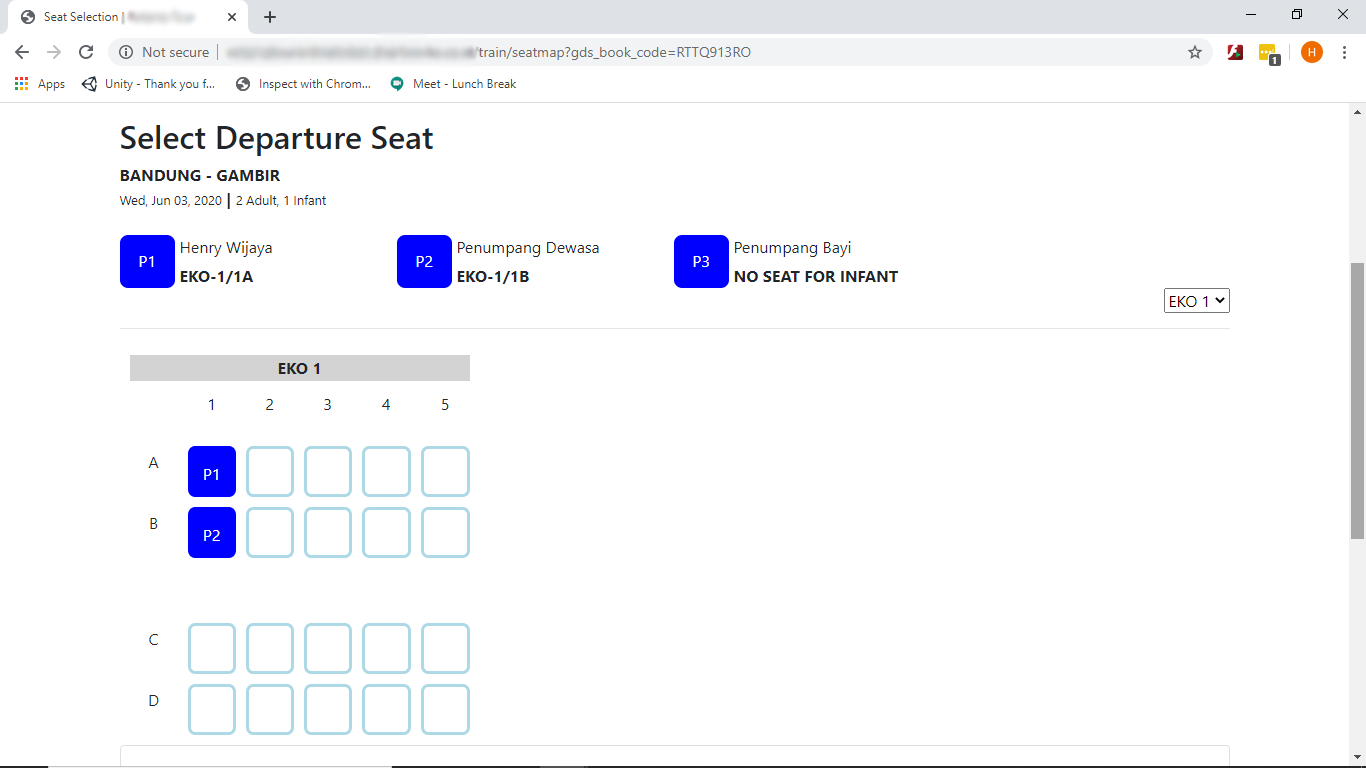
\includegraphics[width=\textwidth,height=\textheight,keepaspectratio]{Gambar/Seat Selection Depart.png}
        \caption{Halaman Pemilihan Kursi.}
            \label{img:pilihkursi1}
        \end{figure}


Fungsi pertama menggunakan hasil 2 modul \textit{API} yang didapat dari \textit{Train\_model}. Modul pertama yang dipakai adalah mendapatkan informasi pemesanan yang contoh isinya dapat dilihat di \ref{subsec:getbookinfo}. Informasi jadwal dan data penumpang bisa didapatkan dari modul ini yang kemudian akan ditampilkan di bagian atas halaman pemilihan kursi. Modul kedua yang digunakan adalah mendapatkan informasi bentuk pemetaan kursi kereta. Contoh hasil dari modul ini dapat dilihat di \ref{subsec:getrailseatmap}. Dari hasil olahan data modul tersebut, peta kursi dapat digambar secara dinamis di \textit{view}.

Fungsi kedua adalah mengganti pilihan kursi penumpang. Jika data kursi penumpang yang diterima di fungsi ini berbeda dengan yang didapat di awal, maka permintaan perubahan kursi akan dikirim ke \textit{server}. Fungsi ini mengirim permintaan mengganti kursi menggunakan modul ketiga yang ditambahkan ke \textit{Train\_model}. Setelah kursi berhasil diganti, pengguna akan diarahkan ke halaman konfirmasi.

\textit{View} untuk halaman ini menampilkan data jadwal yang dipilih dan data penumpang yang didapatkan dari fungsi pertama \textit{controller}. Peta kursi yang digunakan pengguna untuk memilih kursi juga digambar di \textit{view} menggunakan data yang diterima sesuai penjelasan sebelumnya. Bagaimana pengguna memilih kursi diatur juga di \textit{view} ini. Tidak seperti halaman lainnya, \textit{view} ini dibuat dari awal karena halaman ini tidak ada di bagian penerbangan.

Peta kursi digambar dan dihias menggunakan fitur CSS dasar. Seperti yang dapat dilihat pada gambar \ref{img:legendsseat}, terdapat penjelasan untuk masing-masing warna kursi. Tulisan putih P1 pada kotak menunjukkan bahwa kursi itu adalah kursi penumpang 1. Warna biru menunjukkan tempat duduk penumpang saat itu. Warna biru tua adalah kursi yang dipilih saat itu oleh pengguna. Warna putih adalah kursi yang dapat dipilih. Warna abu-abu menunjukkan kursi yang sudah terambil.

\begin{figure}[H]
        \center
        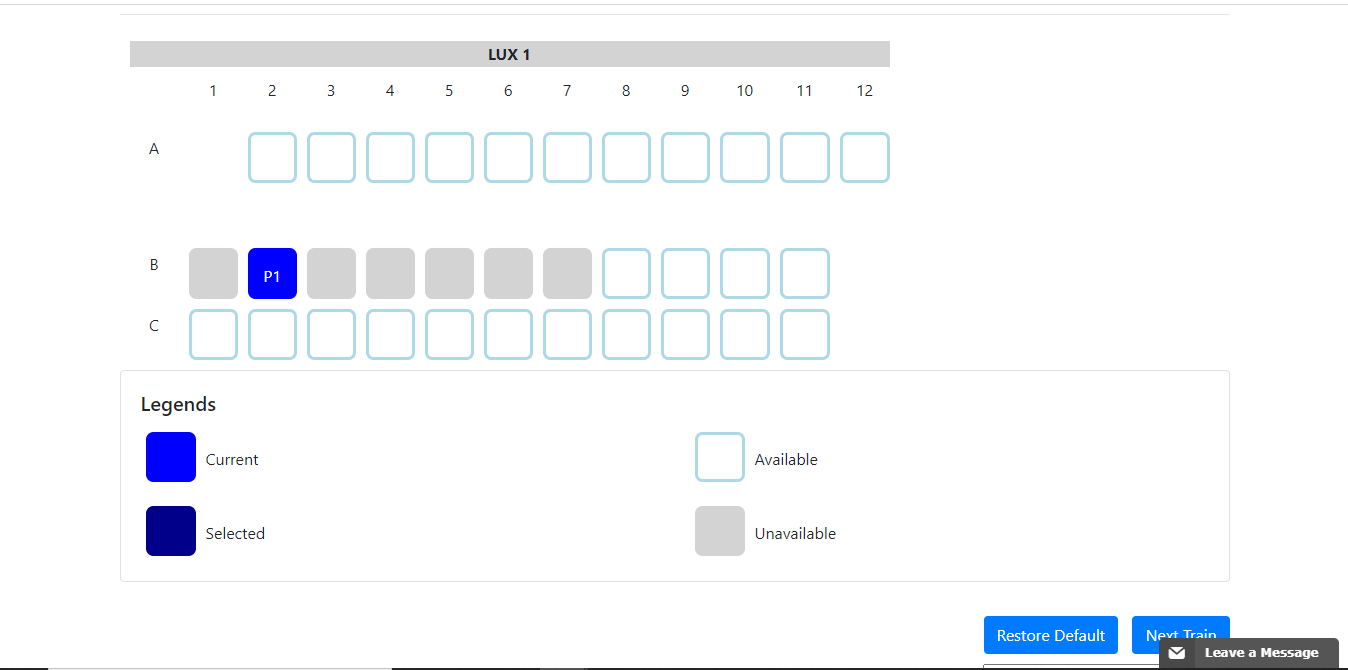
\includegraphics[width=\textwidth,height=\textheight,keepaspectratio]{Gambar/Legends Seat Selection.png}
        \caption{Penjelasan \textit{Icon} Pemilihan Kursi.}
            \label{img:legendsseat}
        \end{figure}

Pengguna bisa memilih kursi dengan mengklik langsung kotak putih pada peta kursi. Pengguna juga bisa memilih gerbong dengan \textit{dropbox} wagon. Setelah diklik, kotak akan berubah warna menjadi biru tua dengan tulisan putih penumpang seperti yang bisa dilihat di gambar \ref{img:penggunapilihkursi}. Pengguna hanya bisa memilih sejumlah penumpang dewasa yang memesan. 

\begin{figure}[H]
        \center
        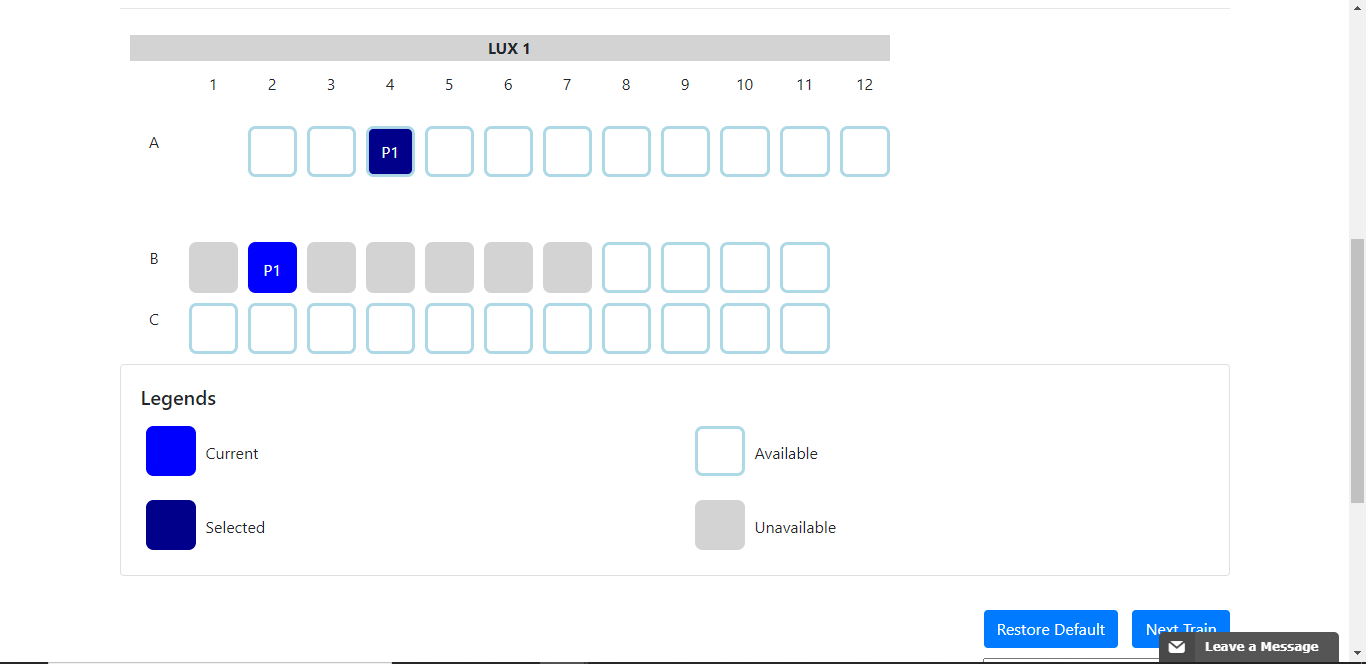
\includegraphics[width=\textwidth,height=\textheight,keepaspectratio]{Gambar/Seat selected.png}
        \caption{Pengguna Memilih Kursi.}
            \label{img:penggunapilihkursi}
        \end{figure}


Jika pengguna berubah pikiran atau salah memilih, pengguna bisa menggunakan tombol \textit{restore default} untuk mengembalikan peta kursi ke kondisi awal. Jika pengguna sudah selesai memilih pengguna bisa menekan tombol \textit{next} atau \textit{next train}. Tombol \textit{next} atau \textit{next train} bergantung pada perjalanan satu arah atau pulang pergi seperti pada halaman-halaman sebelumnya. Tombol \textit{back} yang muncul jika pengguna memilih perjalanan dua arah tidak akan menghapus pilihan pengguna jadi pengguna tetap harus menggunakan tombol \textit{restore default} jika ingin mengganti pilihan.

\section{Konfirmasi dan Pembayaran}
\label{sec:konfirmasidanpembayaran}

Halaman konfirmasi menampilkan data-data yang sudah dipilih penumpang sebelumnya. Data tersebut adalah data jadwal, jumlah penumpang, total harga, dan informasi masing-masing penumpang. Di bagian bawah, terdapat tombol \textit{next} yang akan mengarahkan pengguna ke halaman pembayaran.

Halaman pembayaran ini adalah halaman eksternal yang ditangani oleh \textit{Midtrans}. Di halaman pembayaran ini, pengguna dapat memverifikasi kembali pesanan sebelum membayar. Pengguna dapat memilih metode pembayaran yang pengguna inginkan. Setelah pembayaran dilakukan, transaksi dari sisi pengguna sudah selesai.

\textit{Model} dalam halaman ini menggunakan modul \textit{transaction/payment-new} untuk memberi tahu \textit{server} kalau pengguna sudah bayar. Selain modul dari \textit{API} GDS, \textit{model} juga memiliki fungsi pembuatan \textit{receipt} untuk digunakan di tempat lain seperti \textit{receipt model} dan \textit{midtrans model}. \textit{Receipt} dan \textit{midtrans} model adalah model yang sudah ada sebelum pengembangan modul kereta api. \textit{Model} ini membantu proses pembayaran dengan membuatkan \textit{receipt} transaksi dan komunikasi dengan \textit{API Midtrans}.

Ada dua fungsi yang ditambahkan pada \textit{controller} untuk halaman ini. Fungsi pertama adalah untuk menampilkan informasi-informasi untuk dikonfirmasi oleh pengguna. Fungsi kedua adalah fungsi untuk melakukan pembayaran yang berhubungan dengan \textit{controller Midtrans}. \textit{Controller Midtrans} yang sudah dipakai di bagian penerbangan akan dimanfaatkan kembali untuk mengurus pembayaran di modul kereta.

Di fungsi pertama, informasi disiapkan untuk ditampilkan ke \textit{view}. Informasi yang ditampilkan adalah detail pemesanan dan data penumpang. Detail pemesanan ditampilkan dengan \textit{sidebar} yang sama seperti di \ref{sec:pengisianinfopenumpang}. Detail yang ditampilkan dari atas ke bawah adalah jadwal, jumlah penumpang dan harga. Data penumpang yang ditampilkan oleh fungsi ini adalah nama dan identitas penumpang.

Fungsi kedua akan memanggil \textit{Midtrans\_model} untuk membuat detik transaksi yang akan dikirimkan ke Midtrans. Pengguna akan diarahkan ke halaman Midtrans untuk melakukan verifikasi pesanan dan pembayaran. Setelah melakukan pembayaran, Midtrans akan memberi notifikasi pada sistem kalau pengguna sudah membayar.

Di Midtrans akan memberi notifikasi yang diterima di \textit{controller} Midtrans. Tapi tiket tidak akan langsung di-\textit{issue} karena takut akan dianggap \textit{timeout} oleh Midtrans. \textit{Issue} tiket akan dimasukkan pada \textit{queue} yang akan diproses oleh cron. Cron adalah perangkat lunak yang membantu mengeksekusikan sebuah perintah sesuai jadwal yang sudah ditentukan. Dengan menggunakan cron, maka resiko \textit{timeout} dapat dihindari.